\begin{table*}[t]
\centering
\setlength{\tabcolsep}{3.5pt}
\caption{Main spreadsheet results across skill-author (evolves the skill) and skill-user (runs it at inference) models. SpreadsheetBench reports Vrf (verified), Soft (problem pass rate), and Hard (task pass rate); WikiTQ and HiTab are out-of-distribution (OOD) table-QA transfer, and $\mathrm{Avg}{=}(\mathrm{ID}_{\mathrm{avg}}{+}\mathrm{OOD}_{\mathrm{avg}})/2$ equally weights in-distribution (ID, SpreadsheetBench) and OOD. Reference rows are absolute scores; evolved rows are signed deltas from the Human-Written (Deepening) or Parametric (Creation) baseline. \textbf{Bold} marks the largest absolute score per column. Per-seed standard deviations are in \cref{tab:main_std}.}
\label{tab:main_v1}
\resizebox{\textwidth}{!}{%
\begin{tabular}{@{}l ccccc ccccc c@{}}
\toprule
& \multicolumn{5}{c}{\textit{Skill User: Qwen3.5-122B-A10B}}
& \multicolumn{5}{c}{\textit{Skill User: Qwen3.5-35B-A3B}}
& \\
\cmidrule(lr){2-6}\cmidrule(lr){7-11}
& \multicolumn{3}{c}{\textit{SpreadsheetBench}} & \multicolumn{2}{c}{\textit{OOD}}
& \multicolumn{3}{c}{\textit{SpreadsheetBench}} & \multicolumn{2}{c}{\textit{OOD}}
& \\
\cmidrule(lr){2-4}\cmidrule(lr){5-6}\cmidrule(lr){7-9}\cmidrule(lr){10-11}
\textbf{Condition}
    & \textbf{Vrf}$\uparrow$ & \textbf{Soft}$\uparrow$ & \textbf{Hard}$\uparrow$ & \textbf{WikiTQ}$\uparrow$ & \textbf{HiTab}$\uparrow$
    & \textbf{Vrf}$\uparrow$ & \textbf{Soft}$\uparrow$ & \textbf{Hard}$\uparrow$ & \textbf{WikiTQ}$\uparrow$ & \textbf{HiTab}$\uparrow$
    & \textbf{Avg}$\uparrow$ \\
\midrule
\multicolumn{12}{l}{\textit{Baseline (absolute scores)}} \\
\quad No Skill
    & 27.67 & 28.90 & 17.57 & 21.50 & 14.42 & 19.00 & 18.00 & 4.60 & 13.33 & 19.12 & 18.19 \\
\quad Human-Written
    & 48.33 & 36.30 & 17.03 & 74.68 & 41.31 & 9.67 & 13.03 & 3.37 & 9.02 & 5.30 & 26.93 \\
\quad Parametric
    & 26.17 & 36.60 & 17.50 & 23.73 & 17.36 & 20.17 & 13.70 & 3.87 & 20.14 & 13.94 & 19.23 \\
\midrule
\multicolumn{12}{l}{\textit{Skill Author: Qwen3.5-122B-A10B}} \\[2pt]
\multicolumn{12}{l}{\quad\textit{Deepening (Delta from init: Human-Written)}} \\
\quad\quad +Error
    & \cellcolor{Green3!46}+17.50 & \cellcolor{Green3!57}+10.30 & \cellcolor{Green3!50}+10.40 & \cellcolor{Green3!2}+1.62 & \cellcolor{Green3!5}+2.14 & \cellcolor{Green3!60}\textbf{+27.00} & \cellcolor{Green3!39}+9.44 & \cellcolor{Green3!24}+2.86 & \cellcolor{Green3!13}+9.26 & \cellcolor{Green3!16}+9.55 & \cellcolor{Green3!30}+9.28 \\
\quad\quad +Success
    & \cellcolor{Green3!47}+18.00 & \cellcolor{Green3!47}+8.60 & \cellcolor{Green3!42}+8.70 & \cellcolor{Red1!11}-10.35 & \cellcolor{Red1!2}-0.95 & \cellcolor{Green3!44}+19.66 & \cellcolor{Green3!28}+6.84 & \cellcolor{Green3!11}+1.33 & \cellcolor{Green3!17}+12.09 & \cellcolor{Green3!37}+22.33 & \cellcolor{Green3!26}+8.15 \\
\quad\quad +Combined
    & \cellcolor{Green3!57}\textbf{+21.50} & \cellcolor{Green3!60}\textbf{+10.87} & \cellcolor{Green3!60}\textbf{+12.50} & \cellcolor{Green3!5}+4.56 & \cellcolor{Green3!6}+2.97 & \cellcolor{Green3!47}+21.16 & \cellcolor{Green3!37}+8.84 & \cellcolor{Green3!15}+1.80 & \cellcolor{Green3!9}+6.64 & \cellcolor{Green3!20}+11.94 & \cellcolor{Green3!31}+9.65 \\[2pt]
\multicolumn{12}{l}{\quad\textit{Creation (Delta from init: Parametric)}} \\
\quad\quad +Error
    & \cellcolor{Green3!60}+22.83 & \cellcolor{Green3!21}+3.77 & \cellcolor{Green3!28}+5.87 & \cellcolor{Green3!8}+7.89 & \cellcolor{Red1!4}-1.70 & \cellcolor{Green3!19}+8.66 & \cellcolor{Green3!39}+9.53 & \cellcolor{Green3!33}+4.00 & \cellcolor{Green3!3}+2.06 & \cellcolor{Green3!16}+9.64 & \cellcolor{Green3!22}+6.79 \\
\quad\quad +Success
    & \cellcolor{Green3!40}+15.33 & \cellcolor{Red1!5}-0.93 & \cellcolor{Green3!21}+4.33 & \cellcolor{Green3!25}+23.70 & \cellcolor{Green3!42}+19.89 & \cellcolor{Green3!29}+12.83 & \cellcolor{Green3!48}+11.57 & \cellcolor{Green3!51}+6.13 & \cellcolor{Green3!42}+30.36 & \cellcolor{Green3!48}\textbf{+28.90} & \cellcolor{Green3!55}+16.96 \\
\quad\quad +Combined
    & \cellcolor{Green3!37}+14.00 & \cellcolor{Red1!3}-0.63 & \cellcolor{Green3!17}+3.53 & \cellcolor{Green3!34}+32.32 & \cellcolor{Green3!49}+23.11 & \cellcolor{Green3!34}+15.50 & \cellcolor{Green3!60}\textbf{+14.50} & \cellcolor{Green3!60}\textbf{+7.23} & \cellcolor{Green3!41}+29.70 & \cellcolor{Green3!46}+27.71 & \cellcolor{Green3!60}+18.62 \\[2pt]
\midrule
\multicolumn{12}{l}{\textit{Skill Author: Qwen3.5-35B-A3B}} \\[2pt]
\multicolumn{12}{l}{\quad\textit{Deepening (Delta from init: Human-Written)}} \\
\quad\quad +Error
    & \cellcolor{Green3!44}+16.67 & \cellcolor{Green3!47}+8.50 & \cellcolor{Green3!39}+8.14 & \cellcolor{Red1!7}-6.36 & \cellcolor{Red1!5}-2.38 & \cellcolor{Green3!39}+17.33 & \cellcolor{Green3!38}+9.17 & \cellcolor{Green3!40}+4.83 & \cellcolor{Green3!4}+2.71 & \cellcolor{Green3!13}+8.08 & \cellcolor{Green3!18}+5.64 \\
\quad\quad +Success
    & \cellcolor{Green3!6}+2.17 & \cellcolor{Green3!15}+2.73 & \cellcolor{Green3!16}+3.30 & \cellcolor{Green3!2}+1.46 & \cellcolor{Green3!4}+1.70 & \cellcolor{Green3!27}+12.33 & \cellcolor{Green3!24}+5.87 & \cellcolor{Green3!10}+1.23 & \cellcolor{Green3!60}\textbf{+43.23} & \cellcolor{Green3!57}+34.70 & \cellcolor{Green3!40}+12.44 \\
\quad\quad +Combined
    & \cellcolor{Green3!18}+6.67 & \cellcolor{Green3!21}+3.87 & \cellcolor{Green3!20}+4.17 & \cellcolor{Green3!3}+2.65 & \cellcolor{Green3!5}+2.44 & \cellcolor{Green3!44}+20.00 & \cellcolor{Green3!24}+5.77 & \cellcolor{Green3!20}+2.36 & \cellcolor{Green3!59}+42.20 & \cellcolor{Green3!60}+36.46 & \cellcolor{Green3!45}\textbf{+14.04} \\[2pt]
\multicolumn{12}{l}{\quad\textit{Creation (Delta from init: Parametric)}} \\
\quad\quad +Error
    & \cellcolor{Green3!3}+1.00 & \cellcolor{Red1!43}-7.70 & \cellcolor{Green3!5}+1.03 & \cellcolor{Green3!60}\textbf{+57.65} & \cellcolor{Green3!60}\textbf{+28.25} & \cellcolor{Green3!9}+3.83 & \cellcolor{Green3!30}+7.30 & \cellcolor{Green3!22}+2.66 & \cellcolor{Green3!18}+12.66 & \cellcolor{Green3!29}+17.81 & \cellcolor{Green3!49}+15.22 \\
\quad\quad +Success
    & \cellcolor{Green3!14}+5.33 & \cellcolor{Red1!25}-4.57 & \cellcolor{Green3!12}+2.43 & \cellcolor{Green3!9}+9.09 & \cellcolor{Green3!5}+2.34 & \cellcolor{Green3!13}+5.66 & \cellcolor{Green3!24}+5.80 & \cellcolor{Green3!22}+2.63 & \cellcolor{Green3!5}+3.31 & \cellcolor{Green3!31}+18.94 & \cellcolor{Green3!18}+5.65 \\
\quad\quad +Combined
    & \cellcolor{Green3!22}+8.33 & \cellcolor{Red1!32}-5.83 & \cellcolor{Green3!10}+2.00 & \cellcolor{Green3!32}+30.82 & \cellcolor{Green3!36}+16.93 & \cellcolor{Green3!10}+4.33 & \cellcolor{Green3!40}+9.73 & \cellcolor{Green3!39}+4.73 & \cellcolor{Green3!25}+18.00 & \cellcolor{Green3!42}+25.22 & \cellcolor{Green3!43}+13.31 \\[2pt]
\bottomrule
\end{tabular}
}%
\end{table*}


\section{Experiments}
\label{sec:experiments}

\subsection{Experimental Setup}
\label{sec:experiments:setup}

\myparagraph{Spreadsheet setup.}
Our main experiments use SpreadsheetBench-Verified \citep{ma2024spreadsheetbenchchallengingrealworld}, where agents manipulate \texttt{xlsx} files through tool use.
We split its 400 samples into 200 evolution problems and 200 held-out test problems, and also report Soft/Hard scores on full SpreadsheetBench (excluding all evolving-set problems) plus OOD transfer to WikiTableQuestions \citep{pasupat2015compositionalsemanticparsingsemistructured} and HiTab \citep{cheng-etal-2022-hitab} converted into spreadsheet format.
All spreadsheet results are averaged over three random seeds using each benchmark's official evaluation criteria.

\myparagraph{Skill settings.}
We compare \textbf{No Skill}, the Anthropic \texttt{xlsx} skill (\textbf{Human-Written}), LLM-generated skills using \textbf{Parametric} knowledge, and three \systemname{} variants: \textbf{+Error}, \textbf{+Success}, and \textbf{+Combined}, which consolidate patches from failed trajectories only, from successful trajectories only, and from all trajectories, respectively.
% \textbf{+Error} consolidates patches from failed trajectories, \textbf{+Success} consolidates reusable behaviors from successful trajectories, and \textbf{+Combined} merges both evidence sources.
\textit{Skill Deepening} starts from Human-Written, while \textit{Skill Creation} starts from Parametric.
We evaluate Qwen3.5-122B-A10B and Qwen3.5-35B-A3B as both skill authors and skill users. We do 100\% self-evolution: the same model generates trajectories, proposes patches, and edits skills.
Details of dataset construction, scoring, and model serving are in \cref{app:experimental_details}; the external \texttt{skill-creator} baseline is in \cref{app:skill_creator_baseline}.

\subsection{Main Results}
\label{sec:experiments:main}

\cref{tab:main_v1} reports all spreadsheet results across skill conditions, author models, user models, and transfer tasks.
Baseline rows give absolute scores; evolved rows give signed deltas from the relevant baseline, with Deepening compared to Human-Written and Creation compared to Parametric.
We use \textbf{Avg} as the primary summary metric because it equally weights ID and OOD performance across both user models, rewarding skills that generalize across models and tasks.

\myparagraph{Baselines reveal why both settings matter.}
Human-Written is a useful handcrafted prior, but it is not reliably portable across model scales; Parametric remains close to No Skill, confirming that parametric knowledge alone does not yield actionable spreadsheet skills \citep{han2026sweskillsbenchagentskillsactually}.
These baselines motivate the two evaluation regimes: Deepening tests whether a strong manual skill can be made more transferable, while Creation tests whether trajectory-grounded distillation can build a useful skill from a weak seed.

\myparagraph{Both Deepening and Creation produce generalizable skills.}
Starting from Human-Written, evolved skills consistently strengthen in-distribution spreadsheet performance and often transfer to other model scales and OOD table tasks; starting from Parametric, Creation can match or exceed Human-Written quality in favorable settings.
The gains are broad: they appear across author models, user models, and task families, not only on the model that produced the traces.
Notably, 35B Deepening +Combined attains the best absolute Avg, showing that skills authored by a small LLM can also generalize.
Across analysts, both +Error and +Success help spreadsheet tasks, and +Combined usually gives the largest Avg improvement.

\subsection{Model-Family Generalization}
\label{sec:experiments:model_family}

\begin{figure}[t]
    \centering
    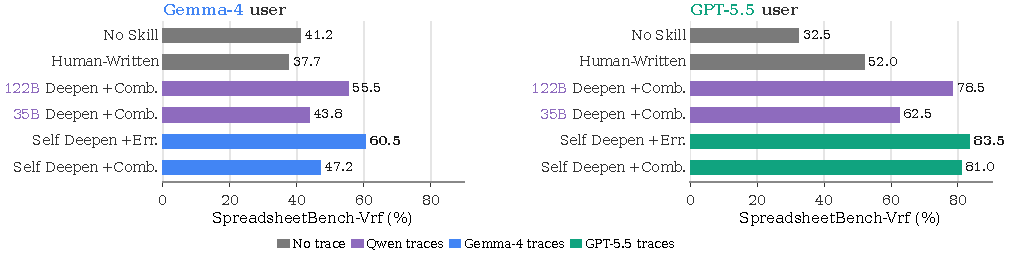
\includegraphics[width=0.96\linewidth]{figures/fig_model_family_generalization.pdf}
    \caption{Cross-family generalization on SpreadsheetBench. Gemma-4-31B-it and GPT-5.5-high each (i)~evolve a skill from their own traces and (ii)~run Qwen3.5-authored skills.}
    \label{fig:model_family_generalization}
\end{figure}

We test generalization across model families with Gemma-4-31B-it and GPT-5.5-high in two settings: each model (i)~deepens the human-written \texttt{xlsx} skill from its own traces via \systemname{}, and (ii)~runs the Qwen3.5-122B/35B +Combined deepened skills. \cref{fig:model_family_generalization} shows that both models self-improve from their own traces and also benefit from Qwen3.5-authored skills, so \systemname{} generalizes across families. \cref{app:model_family_cross_trace} reports additional results and implementation details.


\begin{table}[!t]
\centering
\begin{minipage}[t]{0.48\linewidth}
\centering
\small
\setlength{\tabcolsep}{2.2pt}
\caption{Math transfer to held-out DAPO and AIME. D-Test is DAPO-Math-Test pass rate; AIME is avg@8.}
\label{tab:math}
\resizebox{\linewidth}{!}{%
\begin{tabular}{@{}l cc cc@{}}
\toprule
& \multicolumn{2}{c}{\textit{Skill User: 122B}}
& \multicolumn{2}{c}{\textit{Skill User: 35B}} \\
\cmidrule(lr){2-3}\cmidrule(lr){4-5}
\textbf{Condition}
    & \textbf{D-Test}$\uparrow$
    & \textbf{AIME}$\uparrow$
    & \textbf{D-Test}$\uparrow$
    & \textbf{AIME}$\uparrow$ \\
\midrule
\multicolumn{5}{l}{\textit{Reference (absolute scores)}} \\
\quad No Skill
    & 91.0 & 90.4 & 89.0 & 83.3 \\
\midrule
\multicolumn{5}{l}{\textit{Skill Author: Qwen3.5-122B-A10B}} \\[2pt]
\multicolumn{5}{l}{\quad\textit{Creation (init: No Skill)}} \\
\quad\quad +Error
    & \cellcolor{Green3!60}\textbf{+4.0} & \cellcolor{Green3!60}\textbf{+2.9} & \cellcolor{Green3!50}+5.0 & \cellcolor{Green3!55}+5.0 \\
\quad\quad +Success
    & \cellcolor{Green3!30}+2.0 & \cellcolor{Green3!8}+0.4 & \cellcolor{Green3!20}+2.0 & \cellcolor{Green3!50}+4.6 \\
\quad\quad +Combined
    & \cellcolor{Green3!45}+3.0 & \cellcolor{Red1!25}-1.2 & \cellcolor{Green3!60}\textbf{+6.0} & \cellcolor{Green3!60}\textbf{+5.5} \\[2pt]
\midrule
\multicolumn{5}{l}{\textit{Skill Author: Qwen3.5-35B-A3B}} \\[2pt]
\multicolumn{5}{l}{\quad\textit{Creation (init: No Skill)}} \\
\quad\quad +Error
    & \cellcolor{Green3!45}+3.0 & \cellcolor{Green3!27}+1.3 & \cellcolor{Green3!40}+4.0 & \cellcolor{Green3!5}+0.5 \\
\quad\quad +Success
    & \cellcolor{Red1!20}-1.0 & \cellcolor{Red1!25}-1.2 & +0.0 & \cellcolor{Red1!13}-1.2 \\
\quad\quad +Combined
    & \cellcolor{Green3!15}+1.0 & \cellcolor{Red1!8}-0.4 & \cellcolor{Green3!10}+1.0 & +0.0 \\
\bottomrule
\end{tabular}
}%

\end{minipage}\hfill
\begin{minipage}[t]{0.48\linewidth}
\centering
\small
\setlength{\tabcolsep}{2.2pt}
\caption{DocVQA transfer from trajectory-distilled visual-reasoning skills. ANLS is similarity; Acc is ANLS\,$\ge$\,0.5.}
\label{tab:vqa}
\resizebox{\linewidth}{!}{%
\begin{tabular}{@{}l cc cc@{}}
\toprule
& \multicolumn{2}{c}{\textit{Skill User: 122B}}
& \multicolumn{2}{c}{\textit{Skill User: 35B}} \\
\cmidrule(lr){2-3}\cmidrule(lr){4-5}
\textbf{Condition}
    & \textbf{ANLS}$\uparrow$
    & \textbf{Acc}$\uparrow$
    & \textbf{ANLS}$\uparrow$
    & \textbf{Acc}$\uparrow$ \\
\midrule
\multicolumn{5}{l}{\textit{Reference (absolute scores)}} \\
\quad No Skill
    & 0.6300 & 70.27 & 0.6582 & 73.17 \\
\midrule
\multicolumn{5}{l}{\textit{Skill Author: Qwen3.5-122B-A10B}} \\[2pt]
\multicolumn{5}{l}{\quad\textit{Creation (init: No Skill)}} \\
\quad\quad +Error
    & \cellcolor{Green3!46}+0.1949 & \cellcolor{Green3!48}+17.69 & \cellcolor{Green3!47}+0.1974 & \cellcolor{Green3!45}+16.64 \\
\quad\quad +Success
    & \cellcolor{Green3!39}+0.1639 & \cellcolor{Green3!40}+14.89 & \cellcolor{Green3!40}+0.1668 & \cellcolor{Green3!38}+14.23 \\
\quad\quad +Combined
    & \cellcolor{Green3!60}\textbf{+0.2534} & \cellcolor{Green3!60}\textbf{+22.25} & \cellcolor{Green3!49}+0.2049 & \cellcolor{Green3!46}+17.22 \\[2pt]
\midrule
\multicolumn{5}{l}{\textit{Skill Author: Qwen3.5-35B-A3B}} \\[2pt]
\multicolumn{5}{l}{\quad\textit{Creation (init: No Skill)}} \\
\quad\quad +Error
    & \cellcolor{Green3!21}+0.0884 & \cellcolor{Green3!18}+6.79 & \cellcolor{Green3!30}+0.1267 & \cellcolor{Green3!27}+10.15 \\
\quad\quad +Success
    & \cellcolor{Green3!37}+0.1572 & \cellcolor{Green3!39}+14.53 & \cellcolor{Green3!50}+0.2132 & \cellcolor{Green3!49}+18.27 \\
\quad\quad +Combined
    & \cellcolor{Green3!23}+0.0958 & \cellcolor{Green3!21}+7.73 & \cellcolor{Green3!51}\textbf{+0.2158} & \cellcolor{Green3!51}\textbf{+18.83} \\
\bottomrule
\end{tabular}
}%

\end{minipage}
\end{table}

\subsection{Math Reasoning}
\label{sec:experiments:math}
We apply \systemname{} to math domain to test its domain-agnosticism.
As in the spreadsheet setting (\cref{sec:experiments:setup}), the math agent runs in a ReAct loop with a command-line Python interpreter to write and execute code for each question.
We create skills from scratch on 400 DAPO questions \citep{yu2025dapo} and evaluate on 100 disjoint held-out DAPO questions (ID) and AIME~2026 (OOD competition mathematics; avg@8 over 30 problems), following the cross-model protocol of \cref{sec:experiments:main}.
\cref{tab:math} reports deltas from No Skill.
\textbf{\systemname{} works for math domain:} the distilled skills improve both held-out DAPO and OOD AIME rather than overfitting the source distribution.
\textbf{+Error is the most stable signal}, transferring cleanly between the 122B and 35B users.

\subsection{Visual Question Answering}
\label{sec:experiments:vqa}

To test multimodal generalization, we apply \systemname{} to DocVQA~\citep{mathew2020docvqa}, where agents answer questions over document images such as forms, tables, invoices, letters, and reports.
Again, each agent runs in a ReAct loop with a command-line + Python environment.
We use 50 DocVQA examples only for skill evolution and remove them from evaluation; the remaining 5{,}299 examples form the held-out test set.
We report the official ANLS and Accuracy (ANLS~$\geq 0.5$, \%) for both same-model use and cross-model transfer between 122B- and 35B-authored skills. Results in \cref{tab:vqa} show that \textbf{all
evolved DocVQA skills improve performance over No Skill. +Combined is the strongest setting}, giving the clearest same-model gains and positive cross-model transfer.

% Each VQA agent operates in a ReAct loop (up to 20 turns) with a code-execution tool and a benchmark-specific system prompt.
% We compare two skill conditions:
% \textbf{No Skill} (system prompt only) and
% \textbf{+Evolved} (a skill automatically produced by the closed-loop pipeline: error analysis on the evolving set $\to$ parallel MapReduce skill evolution $\to$ programmatic application).

\FloatBarrier
